\documentclass{scrartcl}
\usepackage[]{geometry}
% \usepackage[parfill]{parskip}
\usepackage[utf8]{inputenc}
\usepackage{graphicx}
    
\usepackage{amsmath,amssymb,amsfonts,amsthm}
\usepackage{chronology}

\usepackage{hyperref}
\hypersetup{
    colorlinks,
    linkcolor=black,
    citecolor=black,
    urlcolor=black,
    linktoc=all,
    }

\begin{document}
\pagestyle{empty}


\tableofcontents
\newpage


\section*{General notes}
\begin{itemize}
\item Goal of supervised learning: predict not yet observed input
\item Motivation: ``\emph{It is probable that no universal beat tracking model exist which does not utilise a switching model to recognize style and context prior to application.}'' \cite[Collins2006]{Collins2006}
\item Instead of calculating the STFT as for input featuress discover a good set of features by representation learning. (``\emph{Learned representations often result in much better performance than can be obtained with hand-designed representations.}'' \cite[Goodfellow2016]{Goodfellow2016})
\item Common association between sequence modeling and recurrent networks: ``\emph{Given a new sequence modeling task or dataset, wich architecture should one use?}'' \cite[Bai2018]{Bai2018}
\item Certain convolutional architectures can reach state-of-the-art accuracy in audio synthesis (e.g. Google WaveNet \cite[Oord2016]{Oord2016})
\item Do TCNs outperform LSTM architectures in this particular sequence modeling task?
\item Contrast of the two statements:
\begin{itemize}
\item ``\emph{Feature extraction is an essential step towards efective and accurate beat/downbeat positions extraction.}'' \cite[Khadkevich2012]{Khadkevich2012}
\item ``\emph{The system shows state-of-the-art beat and downbeat tracking performance on a wide range of different musical genres and sryles. It does so ny avoiding hand-crafted features such as harmonic changes, or rhythmic patterns, but rather leans the relevant features directly from audio.}'' \cite[Boeck2016b]{Boeck2016b}
\end{itemize} 
\end{itemize}

\newpage


\section{Introduction}

\begin{itemize}
\item A fundamental research topic in music information retrieval is the automatic extraction of beat locations from music signals. 
\item The aim of a beat tracker is to recover a sequence of time instants from a musical input that are consitent with the times when a human might tap their foot. \cite{Ellis2007}
\item Beat tracking is an important initioal step in computer emulation of human musc understanding, since beats are fundamental to the perception of (Western) music.
\item The goal of beat tracking is to construct a computational algorithm capable of extracting a symbolic representation which correspond to the phenomenal experience of beat or pulse in a human listener.
\item The primary information required for beat tracking is the onset times of musical events, i.e., musical notes and percussive sounds, and this is sufficient for music of low complexity and litle variation in tempo.
\item The interpretation of beat is on of the most fundamental aspects of musical intelligence.
\item A naive approach to describe the rhythm of musical data is to specify an exhaustive and accurate list of onset times, maybe together with some other musical features characterising those event, e.g., durations, pitches and intensitues. However, such a representations lacks abstraction. Diverse media used for rhyth transmission suffer a trade-off between the level of abstraction and the comprehensiveness of the representation. Standard (Western) music notation provites an accepted method for communication a composition to a performer, but it has little vale in representing the interpretation of a work as played in a caonter. On the other hand, an acoustic signal implicitly contains all rhythmic aspects but provides no abstraction whatsoever \cite{Gouyon2005}.
\item The main goal in automatic rhythm desciption is the parsing of acoustic events that occur in time into the more abstract notions of metrical structure, tempo and timing. A major difficulty is the inherent ambiguity of rhythm, as discussed in section \ref{sec:difficulties}.
\item How well does the proposed model gneralise to different musical styles?
\end{itemize}




\subsection{Difficulties of Beat Tracking}
\label{sec:difficulties}
It is difficult to reliably extract high-level rhythm related features from musical excerpt having properties such as [Quinton2016]
\begin{itemize}
\item The principal reason that beat tracjing is intrinsically difficult is that is is the problem of inferring an original beat strucutre that is not expressed explicitly. The degree of beat tracking difficulty is therefore not determided simply by the number of musical instruents performing a musical piexe it depends on how explicitly the beat structure is expressed in the piece. However, it is very difficult to measure its explicitness because it is influenced from various aspects of the songs.
\item The larger the number of syncopation, the greater the difficulty of beat tracking (quantitative measure: power-difference measure \cite{Goto1999})
\item The main reason that different tendencies with regard to the explicitness with which their beat structure is indicated.
\item There is not necessarily a specific sound that directly indicates tho position of beats. In fact, a musical beat may not directly correspond to a real sound, there may even be no signal on a beat. 
\item absence of a clear rhythmic structure (Classical music)
\item soft onsets
\item blurred note transitions (e.g. classigal music dominated by string instruments)
\item heavy syncopation
\item expressive timing (e.g. rubato playing)
\item the problem of 'octave errors' (detecting double or half time the rate of the ground truth)
\item acoustiv signals consit of sound of various kinds of instruments
\item the onsets of notes are difficult to obtain, unlike the case of MIDI signals, where there is no such problem.
\item a beat may not directly correnspond to a real sound. It is a perceptal concept that human feels in music. 
\item Multiple interpretations of beats are possible at any given time
\item There is no simple relationship beteen polyphonic complexity - the number and timbres of notes played at a single time - in apiece of music, and its rhythmic complexity or pulse complexity \cite{Scheirer1998}. There are pieces and sryles of music which are texturally and timbrally complex, but have straighforward, perceptual simple rhythms; and ther also exist music which deal in less complex textures but are more difficult to rhythmically understand an describe.
\item The complexity of grouping harmonic partials together to form notes, and determining the onst times of those.
\item For this reason Cemgil et al. \cite{Cemgil2001} define music transcription as the extraction of an \emph{acceptable} music notation.
\item Ther is no canonical form for representing rhythm, and lacking this ground truth, it is difficult, if not impossible, to provide a meaningful quantitative comparison of the variuos computer systems. Therefore we need a common database of test music labelled with the ground truth on which the systems are tested. 
\end{itemize}



% Quantify the difficulty of beat tracking with indicators such as
% \begin{itemize}
% \item beat strength [Tzanetakis2002]
% \item pulse clarity [Lartillot2008]
% \item entropy of a cyclic tempogram [Grosche2010] as an indicator of the tempo salience  
% \end{itemize}


\subsection{Applications of Beat Tracking}

\begin{itemize}
\item Beat tracking can be used to automate the time-consuming tasks that must be completed in order to synchronize events with music. 
\item Video and audio editing (visual track can be automatically synchronized with an audio track using beat tracking)
\item Stage light control. In live performances, beat tracking is useful in the control of stage lighting by a computer. For instance, various properties of lighting such as color, brightness, direction, and effect can be changed in time to the music.
\item Visualization for example time-grid in audio sequencers.
\item Musical interaction systems \cite{Robertson2007}
\item Content-based audio effects, for multimedia or interactive performances or studio post-production
\item Beat-driven reat-time computer graphics.
\item Temoral segmentation to higher level MIR tasks such as chord estimation for harmonic description \cite{Bello2005b}.
\item Long-term structural segmentaion of audio \cite{Bartsch2005}
\item performance analysis investigates the interpretation of musical works, e.g., the performer's choice of tempo and expressive timing. 
\item In audio content analysis beat tracking is important for automatic indexing and content-based retrieval of audio data, such as in multimedia databases and libraries.
\item Automatic transcription and score extraction from performance data 
\item Music similarity
\item Beat tracking can provide computers the ability to participate intelligently in live performances in real time and join the ensemble.
\item synchronisation of a musical performance with computers or other devices
\item Commercial devices already exist that attept to extract a MIDI clock from an audio signal, indication both the tempo and the actual location of the beat. Such MIDI clocks can the be used to synchronize other devices such as drum machines or audio effects, enabling a new range of beat-synchronized audio processing.
\item Automatic playlist generation, where a computer is given the task to choose a series of audio tracks from a track database in a way similar to what a human deejay would do. The track tempo is a very important selection criterion in this context, as deejays will tend to string tracks with similar tempi back to back. Furthermore, deejays also tend to perform beat-synchronous crossfading between successive track manualy, slowing down or speeding up one of the tracks so that the beat in the two tracks line up exactly during the crossfade. This can easily be done automatically once the beats are located in the two tracks.
\end{itemize}



\newpage
\section{History of Beat Tracking}

The following chapter is a summary (background) of related work that forstered the development of automatic beat tracking in musical audio.
\begin{itemize}
\item Overview: Signal processing $\rightarrow$ data-driven approaches
\item The task of beat tracking has been well established over the last twenty-five years. 
\item The first analysis step is the creation of a feature list, i.e. the parsing, of filtering, of the data at hand into a sequence of features. These features range from note onset features (as time, duration and pitch), to frae-based signal features, and they convey the predominant information relevant to rhythmic analysis.
\item The extraction of note onsets times for rhythmic analysis is ubiquitous in the litarature. An exhaustive overview of musical onset detection can be found in \cite{Bello2003}.
\item Some systems do not focus on note onsents and their features, but refer to a data granularly of a lower lever of abstraction, namely frames. A frame is a short chunk, typically $10\,\text{ms}$ of audio, from which both time and frequency domain features can be computed. Consecutive frames are usually considered with some overlap for smoother analyses, and the analysis step, the hop size, equals the frame size minus the overlap. 
\end{itemize}

\begin{figure}[htpb]
\centering
\begin{chronology}[5]{1984}{2024}{\textwidth}[\textwidth]
\event{1985}{Schloss \cite{Schloss1985}}
\event{1990}{Allen and Dannenberg \cite{Allen1990}}
\event{1994}{Goto and Muraoka \cite{Goto1994}}
\event{1998}{Scheirer \cite{Scheirer1998}}
\event{2001}{Cemgil et al. \cite{Cemgil2001}, Dixon \cite{Dixon2001}}
\event{2003}{Laroche \cite{Laroche2003}}
\event{2005}{Klapuri et al. \cite{Klapuri2005}} % Lacoste and Eck \cite{Lacoste2005}
\event{2007}{Davies and Plumbley \cite{Davies2007}}
\event{2009}{Peters \cite{Peeters2009}}
\event{2011}{Böck and Schedl \cite{Boeck2011}}
\event{2014}{Böck et al. \cite{Boeck2014}}
\eventmarker{2015}{Krebs et al. \cite{Krebs2015}}
\eventlabel{2016}{Krebs et al. \cite{Krebs2015}}
% \event{\decimaldate{25}{6}{2015}}{Krebs et al. \cite{Krebs2015}}
\event{2019}{Davies and Böck \cite{Davies2019}}


% \event{\decimaldate{25}{6}{2001}}{three}
\end{chronology}

\caption{Timeline with the history of beat tracking.}
\label{fig:figure1}
\end{figure}



% Chowning et al. 1984 /cite{Chowning1984}

The earliest work on automatic extraction of rhythmic contet from audio is published 1985 in the percussion transcription system of Schloss \cite{Schloss1985}. Onsets are detected as peaks in the slope of the amplitude envelope, where the envelope is defined to be equal to the maximum aplitude in each period of the high-pass filterd signal, and the period defined as the inverse of the lowest frequency expected to be present in the signal. The main limitation of the system is that it requires parameters to be set interactively. 

Allen and Dannenberg \cite{Allen1990} extended the musical concept of beat to include two aspects, namely period and phase. Based on that concept, they built a method that uses real-time beam search to allow the beat tracker to consider several possible stages at once. They use a credibility measure so that at any given time there si a set of active states that represent the most credible interpretations for the performance encoutered so far. However, the system's reliance on MIDI limited the input source to electronic instruments, and moreover limeted its application.

Goto and Muraoka \cite{Goto1994} introduce the first worth mentioning beat tracking system which could process music played on ensembles of a variety of instruments. However, they restricted their system to rock and pop music in which drums maintain the the beats. The system leverages the fact that for a large class of popular music, a bass drum and a snare drum usually occur on the strong and weak beats, respectively. It manages multiple agents that track beats according to different stategies in order to examine multiple hypothesis in parallel. All hypotheses are gathered and the most reliable one is selected as the output. This enables the system to follow beats without losing track if them, even if some hypothesis became wrong. Assumptions were made; between 65 and 185 BPM, time-signature is 4/4, tempo stays almost constant. In following developments, Goto present a beat tracking system for both music with and without drum-sounds \cite{Goto2001}. It uses frequency-domain analysis to detect chord cahnges, which are assumed to occur in metrically strong positions. This is the fist system to demonstrate the use of high level information in directing the lower-level beat tracking process. The high level information is specific to the musical style, which is a major limitation of the system.  

Scheirer \cite{Scheirer1998} figured out from psychoacoustic demonstration on beat perception, that amplitude envelopes from a small number of broad frequency channels are sufficient information to rhythmically analyse musical content. He concludes that a rhythmic processing algorithm shoud treat frequency bands separately, combining results at the end, rather than attempting to perform beat tracking on the sum of filterbank outputs. This leads him to the use of a small number of bandpass filters and banks of parallel comb filters, which function as tuned resonators, to perform periodicity analysis. In the next processing step, the phase of the musical siganl is extracted by examining the internal state of the delays of the comb filters. Finally, the phase and the period is used to estimate the beat times as far into the future as desired. One problem with the system is that in order to track tempo changes, the system must repeatedly change its choice of filter, which implies the filters must be closely spaced to be able to smoothly track tempo variations. However, the system applies no continuity constraint when switching between filters.  

% Dixon 2001
Dixon \cite{Dixon2001} processes a sequence of note onset times either extracted from an audio signal or from a symbolic representation within a multi-agent system. Likely tempo hypotheses are derived from clutering inter-onset intervals (IOI), thus encoding aspects of the metical hierarchy. The hypothesis are used to form multiple beat agents using a paradigm, where each agent has a state consiting of the period and the phase of the beat. The sequence of beat times with the best score to date is selected by the agent. The observations are only processed if they occur around the predicted beat locations, i.e., within a window whose width depends on the pulse period. The algorithm is designed to track beats in expressivey performed music.
% add Dixon 2003

% In this framework, 

% \begin{itemize}
% % \item Dixon \cite{Dixon2001} uses histograms of time intervals between similar events. He uses IOI histograms where the bins are not fixed.
% % \item Clusters of similar IOIs are given scores based on the number of elements in the cluster and the amplitudes of ther onsets.
% % \item An ajustment of the scores and cluster representative interval the favours rationally-related cluster
% % \item The computation of the period entails the loss of time localisation, and the phase has to be computed subsequently  during pulse trackking. 
% % \item Uses a fixed tolerance interval of $25\,\text{ms}$ für IOIs
% % \item Presents another multiple hypotheses search, using an agent paradigm, where each agent has a state, consiting of the period and the phase of the pulse, and a history, the sequence of beat times selected to date by the agent. The observations are only processed if they occur around the predicted beat locations, i.e., within a window whose width depends on the pulse period.
% \item Dixon et al. \cite{Dixon2003} employ tolerance intervals proportional to the IOIs, so longer IOIs allow for greater variations.
% \end{itemize} 

Cemgil et al. \cite{Cemgil2001} formulate beat tracking in a Bayesian framework where tempo and beat is modeled as a stochstic dynamical system. The system is defined with two hidden state variables, namely the period and the phase of beat. To this deterministic model, they add a Gausssian random vector whose covariance matrix models the likely tempo variations. State transitions are defined by a simple set of equations that describe how state variables evolve with time. 
Because all noises are assumed to be Gaussian and all relationships between variables are linear, the covariance matrix can be efficiently estimated by a Kalman filter. They also define the tempogram representation which includes a probability distribution over the period and phase given a list of onset. This probability distribution is proportional to the likelihood of the observed onsets under given period and phase hypotheses, wheighted by prior distribution, which is equally distributed, as they consider all tempi to be initially equiprobable. For given periods and phases, the likelihood is computed as the integral over all onsets of the product of a constant pulse track and a continous representation of the onsets. This implements the assuption that a good pulse track is one which matches all onsets well. The tempogram marginal probability distribution $p(\omega | t)$ provides a 1-D representation of periodicities resembling those aforementioned. 
 %  will be estimated through a training phase.



% Temperley and Sleater \cite{Temperley1999} use dynamic programming to search the solution space of possible mappings of events to a metrical grid, where the search is guided by a set of preference rules based of GTTM.


Laroche \cite{Laroche2003} initially finds salient features like note onsets, note changes, and percussion hists by calculating the Fourier transform of an audio signal. A nonlinear monotonic compression function is applied to the amplitude spectrum, so high-frequency components are not masked by higher amplitide low-frequency components. To locate fast variations in the frequency domain contents, a first-order difference is calculated. All bins are summed together, and the result is half-wave rectified to obtain a positice energy flux signal. A least-squares approach is used to determine the best candidates for the tempo and beat locations. The final step consist of going through the successive tempo analysis frames and finding in each frame the best candidates. To that effect a dynamic programming techning is used. This entails continuity and non-sysncopation constraints. 


Klapuri et al. \cite{Klapuri2005} expand upon Scheirer's amplitude envelope and comb filter model. They adopt a more robust registral accent signal across four parallel analysis bands as the input to their system and use comb filterbanks within a probabilistic framework to simultaniously track three metrical levels. These correspond to the tatum, tactus and measure, which are explained in section \ref{sec:perception}. Analysis can be performed causally an noncausally, and is not restricted to any particular genre, tempo or time-signature. The robustness of the analysis model is due to the probabilistic modelling of the temporal evolution and interaction between each og the three metrical levels analysed. In a study of audio temoo induction algorhithms \cite{Gouyon2006b}, this approach was shown to be most accurate.


Davies and Plumbley \cite{Davies2007} adopt a simpler and more efficient, heuristic approach than the system of Klapuri by embedding context-dependent information directly into the beat period and alignment estimation processes. They use two state model; the first state performs tempo induction and tracks tempo changes, while the second maintains contextual continuity within a single tempo hypotheseis. The first state, also called general state, operates in a memoryless fashion, extracting the beat period and beat alignment through a process of repeated induction. In this manner, the two-state model can explicitly model tempo discontinuities while smoothing out odd beat errors during each consistent beat period hypothesis. 

Peeters \cite{Peeters2009} approach is based on a probabilistic framework, in which the beat tracking problem is formulated in a hidden Markov model, that can be efficiantly solved with the Viterbi algorithm \cite{Viterbi1967}. An onset-energy-function, time-variable tempo, and meter serves as an input to the system. Beat times are decoded over beat-numbers according to observation and transition probabilities. A beat-template is used to derive the observation probabilities from the signal. For this purpose, a linear discriminant analysis finds the most discriminative beat-template. 
% A significant change was introduced by Eyben who transit from signal processing to data-driven method which utilise the power of machine learning. 


\newpage
% basic principles of how humans understand rhythms
\section{Basic Principles of Human Rhythm Perception}
\label{sec:perception}

\begin{itemize}
\item Beat, as a phenomenon, refers to the perceived pulses which are approximately equally spaced and define the rate at which notes in a piece of music are played. For a specific performance, the beat is defined by the occurance times, beat times, of these pulses.
% \item Metrical level see Dixon 2001
\item Western music notation provides an objective regular temporal structure underlying musical event occurances and organising them into a hierachical metrical structure \cite{Gouyon2005}. 
\item Many works in musicpsychology attempt to group musical onsets together into a rhythmic context, i.e., to construct a model which subsubes multiple onsets separated in time into a rhythmic clock, hierachy, grouping, or oscillatory model.
\item A rhythmic event is characterised by an onset time and a salience. They represent the most basic unit of rhythmic information, from which all beat and tempo information us derived.
\item The more salient events are the more likely to correnspondent to beat times than the less salient events. This tendency for events with greater perceptual salience to occur in stronger metrical positions has been noted by various authors \cite{Lerdahl1985,Povel1985,Parncutt1994}.
\item Each pair of events in arhythmic sequence initially contributes to the salience of a single pulse sensation (emphasis occurs), and later that pulse sensations can enhance the salience of other consonant pulse sensations \cite{Parncutt1994}. One may understand the initially above as an indication not to implement influential schemes beteen metrical levels in the induction process, but imdeed to do it in the tracjing process, which is also in agreement with the Dynamic Attending Theory \cite{Jones1989}.
\item Perception research has shown that with up to $40\,\text{ms}$ difference in onset times, two tones are heard as synchronous, and for more than two tnoes, the threshold is up to $70\,\text{ms}$ \cite{Handel1989}. 
\item Rhythmic information is provided by IOIs in the range of approcimately $50\,\text{ms}$ to $2\,\text{s}$ \cite{Handel1989}.
\item Perception of beat is a prerequisite to rhythm perception, which in turn is a fundamental part of music perception.
\item Experiments on the tempo sensitivity on humans have shown that the ability to notice tempo changes is proportional to the tempo, with the JND (just noticable difference) beeing around 2-5\% \cite{Drake1993}.
\item Although in the brains of performers music is temporally organized according to its hieaechical beat structure, this structure is not explicitly expressed in music; it is implied in the relations among variuos musical elements which are not fixed and which are dependent on musical genres or poeces.
\item A listener who cannot identify chord names can nevertheless percieve chord changes.
\item The experience of rhythm involves movement, regularity, grouping, and yet accentutation and differentiation \cite{Handel1989}.
\item There is no ground thuth for rhythm to be found in simple measurement of an acoustic signal. The only ground truth is what human listeners agree to be the rhythmic aspects of the musical contetent of that signal
\item As contrasted with rhythm in general, beat and and pulse correspond inly th the sense of equally spaced temporal units \cite{Handel1989}. Where meter and rhythm associate with qualities of grouping, hierarchy and a strong/weak dichitimy, pulses in apiece of music are only periodic at a simple level.
\item The Generative Theory of Tonal Music (GTTM) \cite{Lerdahl1985} formalises the distinction objective stucture and the performers conceptualisation of music by defining rules for a ``musical grammar'' which deals separately with grouping structure and metrical structure. While the grouping structure deals with time spans, the metrical structure deals with durationless points in time, the beats, which obey the following rules. Beats must be equally spaced. A division according to a specific duration corresponds to a metrical level. There must be a beat of the the metrical structure for every note in a musical sequence. A beat at a high level must also be a beat at each lower level. At any metrical level, a beat which is also abeat at the next higher level is called a downbeat, and other beats are called upbeats. Beats obey a discrete time grid, with time intervals all being multiples of a common duration the smalles metrical level. 
\item Lerdahl and Jackendoff \cite{Lerdahl1985} describe meter perception as the progress of finding periodicities in the phenomenal and structural accents in a piece of music. They propose a set of metrical preference rules, based on musical intuitions, which are assumed to guide the listener to plausible interpretations of rhythms. The rules prefer structures where: beats coincide with note onsets; string beats coincide with onsets of long notes; parallel groups receive parallel metrical structure; and the strogest beat occurs early in the group.
\item Lerdahl and Jackenhoff \cite{Lerdahl1985} classify musical accents into three types: phenomenal accents, whoich come from physical attributes of the signal such as amplitude and frequency; structural accents, which arise from perceived points of arrival and departure such as cadences; and metrical accents, points in time which are perceived as accented due to their metrical position.
\item A major weakness of the GTTM is that it dows not deal with the departures from stroct metrical timing which are apparent in almost all styles of music. Thus it is only reall suitable for representing the timing structures of musical scores, or as an abstract representation of a performance, where the expressive timing is not represented.
\item Drake and Bertrand \cite{Drake2001} advocate a universal predisposition toward simple duration ratio, and claim that humans thend to hear a time interval as twice as long or short as previous intervals. The Dynamic Attending Theory \cite{Jones1989} proposes that humans spontaneously focus on a reference level of periodicity, and they can later switch to other levels to track events occuring at differnt time spans, e.g., longer span harmony changes, or a particular shorter-span fast motive. 
\item They list the following types of phenomenal accent, which they consider incomplete: note onsets, sforzandi, sudden dynamic or timbral changes, long notes, melodic leaps and harmonic changes. However, they give no indication as to how these factors might be compared or combined, either quantitatively (absolute values) or quanlitatively (relative strengths).
\item Longer notes tend to be perceived as accented.
\item The beat of a piece of music is the sequence of equally spaced phenomenal impulses which define a tempo for the music. 
\item The period of a beat is the time duration between two successive beats, i.e., the reciprocal of the tempo.
\item The phase of a beat determines where a beat occurs with respect to performance time.
\item The frequency pf the pulse in a rhythmic musical signal is the tempo or the rate of the rhythm, and the phase of the pulse indicates where the downbeat of the rhythm occurs. That is, the times at which a pulse occurs can be defined to have zero phase, and thus the points in time exactly in-between pulses hace phase of $\pi$ radians.
\item In order to represent changing tempi, various approaches can be used. If tempo is considered as an instantaneous value, it can be calculated as the inter-beat interval measured between each pair of successive beat. A more preceptual plausible approach is to take an average tempo measured over a longer period of time. A measure of central tendency of tempo over a complete musical excerpt is called the basic tempo \cite{Repp1994}, which is the implied tempo around which the expressive tempo varies.
\item The value of tempo as a function of time is called a tempo curve.
\item Tempogram \cite{Cemgil2000}
\item Given a metrical structure, tempo is defined as the rate of the beats at a given metrical level, for example the quarter note level in the score. 
\item There is usually a preferred or primary metrical level, which corresponds to the rate at which most people would tap or clap in time with the music, and this is commonly used to define the tempo, expressed either as a number of beats per minute, or as the time intercal between beats, the inter-beat interval (IBI).
\item The perception of tempo exhibits a degree of variability. It is not always correct to assume that the denominator of the time signature corresponds to the ``foot-tapping'' rate, nor to the actual ``physical tempo'' that would be an inherent property of audio flows \cite{Drake1999}.
\item Differences in human perception of tempo depend on age, musical training, musical preferences and general listening context, e.g., tempo of a previously heard sequence, listener's activity, instant of the day \cite{Drake1993,Drake2000,Drake2000b}
\item Differences in tempo perception are nevertheless far from random. They most often correspond to a focus on a different metrical level, e.g., differences of half or twice the inter-beat interval or one-third or three times the inter-beat interval. 
\item Human pitch recognition is only sensitive to signal phase under certain unusual conditions. rhythmic response is crucially aphased phenomenon - tapping on the beat is not at all the same as tapping against the beat. or slightly ahead of or behind the beat, even ig the frequency of tapping is accurate \cite{Scheirer1998}
\item From psychoacoustic demonstration on beat perception it can be shown that certain kinds of signal manipulations and simplifications can be performed without affecting the perceived pulse content of a musical signal. An amplitude-modulated noise constructed by vocoding a white noise signal with the subband envelopes of a musical signal is sufficient to extract pulse and meter. The simplified signal is created by performing a frequency analysis of the original signal by processing it through a filterbank of bandpass filters, or grouping FFT bins together. Thus it seems that separating the signal into subbands and maintaining the subband envelopes separately is necessary to do accurate rhythmic processing. This fact leads to the hypotheses that some sort of cross-band ryhtmic integration, not simply summation across frequency bands, is performed by the auditory system to perceive rhythm \cite{Scheirer1998}.
\item Studies of Povel and Essnes \cite{Povel1985} have demonstrated that beat perceptin may be explianed with a model in which a perceptual clock is aligned with the accent structure of the input. The model relies heavily on structural qualities of the input, such as a sophisticated model of temporal accent, to function.
\item They propose a model of perception of temporal patterns, based on the idea that a listener tries to induce an internal clock which matches the distribution of accents in the stimulis and allows the pattern to be expressed in the simplest possible terms. They use patterns of identical tone bursts at precise multiples of $200\, \text{ms}$ apart to test their theory. 
\item Expressive timing is generated from perforers' understanding of the musical structure an general knowledge of music theory and musical style \cite{Clarke1999}. However, there is no precise mathematical model of expressive timing, and the complexity of musical structure fro which timing is derived, coupled with the individuality of each performer and performance, makes it impossible to capture musical nuance in the form of rules \cite{Dixon2001}. 
\item Expressive reductions in tempo are more common and more extreme than tempo increases \cite{Repp1994}. % change transition prob in HMM
\end{itemize}


\newpage
\section{Foundations of Machine Learning}


\subsection{Sequence Modeling}

Given an input sequence $x_{1:T} = x_1, \dots, x_T$ with sequence length $T$, a sequence model is any function $f: \mathcal X^T \rightarrow \mathcal Y^T$ such that
\begin{align}
y_{1:T} = y_1, \dots, y_T = f(x_1,\dots, x_T)
\end{align}
where $y_t$ should only depend on $x_{1:t}$ and not on $x_{t+1:T}$, i.e., no leakage of information from the future. This causality constraint is essential for autoregressive modeling. We use $x_{1:T} = x_1, \dots, x_T$ to denote a input sequence of length $T$, where vector $x_t \in \mathbb R^p$ is the input at time step $t$. Thus $x_{1:T} \in \mathbb R^{T \times p}$.

The goal of learning in the sequence modeling setting is to find a network $f$ that minimizes some expected loss between the actual outputs and the predictions, 
\begin{align}
L \big( y_1, \dots, y_T, \, f(x_1,\dots, x_T) \big) \stackrel{\text{!}}{=} \min
\end{align}
where the sequences and outputs are drawn according some distribution.

For most deep learning practitioners, sequence modeling is synonymous with recurrent networks. For example the sequence modeling chapter in a standard reference on deep learning is titled ``Sequence Modeling: Recurrent and Recursive Nets'' \cite{Goodfellow2016} capturing the common association of sequence modeling and recurrent architectures. Recent results indicate that convolutional architectures can outperform recurrent networks. Concluding from an empirical evaluation of generic convolutional and recurrent networks for sequence modeling, Bai et al. \cite{Bai2018} assert that the common association between sequence modeling and recurrent networks should be reconsidered, and convolutional networks should be regarded as a natural starting point for sequence modeling tasks.


\begin{itemize}
\item Sequence modeling include polyphonic music modeling\cite{Oord2016}, word- and character-level language modeling.
\item settings such as auto-regressive prediction, where we try to predict some signal given its past, by setting the target output to be simply the input shifted by ome time step
\end{itemize}






\subsection{Data Representation}

\begin{itemize}
\item Many artificial intelligence tasks can be solved by designing the right set of features to extraxt for that task, then providing theses features to a simple machine learning algorithm. \cite{Goodfellow2016}
\end{itemize}




\subsection{Architectures}

\begin{itemize}
\item Given a sequence modeling task or dataset, which architecture should one use?
\item Bai et al. \cite{Bai2018} show that a simple convolutional architectures outperforms canonical recurrent networks such as LSTMs across a diverse range of tasks and datasets, while demonstrating longer effective memory. Is it also the case in beat tracking?
\end{itemize}


\subsubsection{Recurrent Neural Networks}

In deep learning, a recurrent neural network (RNN) is a class of artificial neural networks where connections between nodes form a directed graph along a temporal sequence.

\begin{itemize}
\item Recurrent networks are dedicated sequence models that maintain a vector of hidden activations that are propagated throgh time \cite{Elman1990,Werbos1990,Graves2012}.
\item This family of architectures has gained tremendois popilarity die to prominent applications to language modeling and machine translation.
\item The intuitive appeal of recurrent modeling is that the hidden state can act as a representations of everything that has been seen so far in the sequence.
\item Basic RNN architectures are notoriously difficult to train and more elaborate architectures are commonly used instead, such as the LSTM \cite{Hochreiter1997} and the GRU \cite{Cho2014}.
\end{itemize}

\begin{figure}[htbp]
\centering
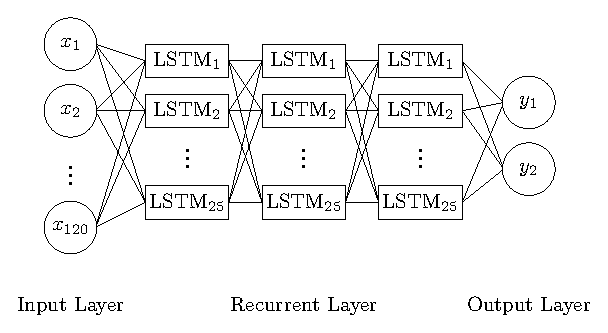
\includegraphics[scale=1.0]{figures/neural_network_boeck.eps}
\caption{Model architecture in \cite{Boeck2011}.}
\label{fig:}
\end{figure}    


\subsubsection{Convolutional Neural Networks}

A convolutional neural network (CNN) is a class of deep neural networks, most commonly applied to analyzing visual imagery.

\begin{itemize}
\item Convolutional neural networks (CNNs) \cite{LeCun1989} have been applied to sequences for decades. They were used prominently for speech recognition in the 80s and 90s.
\end{itemize}



\subsubsection{Temporal Convolutional Netwoks}

A temporal convolutional network (TCN)  represents a special kind of convolutional neural network and is informed by recent convolutional architectures for sequential data \cite{Bai2018}. It is designed from first principles and combines simplicity, autoregressive prediction, and very long memory. In comparison to WaveNet \cite{Oord2016}, the TCN does not employ skip connections across layers (no conditioning, context stacking, or gated activations).

The TCN is based upon two principles: 1) the convolutions are casual, i.e, no information leakage from future to past; 2) the architecture can take a sequence of any length and map it to an output sequence of the same length just as with an RNN. To achieve the first point, the TCN uses a 1D fully-convolutional network architecture \cite{Long2015}, where each hidden layer is the same length as the input layer. To accomplish the second point, the TCN uses causal convolutions, i.e., convolutions where an output at time $t$ is convolved only with elements from time $t$ and earlier in the previous layer.

Simple causal convolutions have the disadvantage to only look back at history with size linear in the depth of the network. To circumvent this fact, the architecture employs dilated convolutions that enable an exponentially large receptive field. More formally, for a 1-D sequence input $\mathbf x \in \mathbb R^T$ and a filter $f:\{ 0, \dots, k-1\} \rightarrow \mathbb R$, the delated convolution operation $F$ on element $s$ of the sequence is defined as
\begin{align}
F(s) = (\mathbf x *_d f)(s) = \sum_{i=0}^{k-1} f(i) \, \mathbf x_{s-d\cdot i}
\end{align}
where $d = 2^\nu$ is the dilation factor, with $\nu$ the level of the network, and $k$ is the filter size. The term $s-d\cdot i$ accounts for the direction of the past. Dilation is equivalent to introducing a fixed  step between every two adjacent filter taps, as it can be seen in Fig. \ref{fig:dilated_convolutions}. Using larger dilation enables an output at the top level to represent a wider range of inputs, thus effectivly expanding the receptive field of a CNN. There are two ways to increase the receptive field of a TCN: choosing lager filter sizes $k$ and increasing the dilation factor $d$, since the effective history of one layer is $(k-1) \, d$. 
\begin{figure}[htbp]
    \centering
    \includegraphics[]{figures/tcn_dilated_casual_convolution.pdf}
    \caption{A dilated casual convolution with dilation factors $d = 1,2,4$ and filter size $k=3$ \cite{Bai2018}.}
    \label{fig:dilated_convolutions} 
\end{figure}

Another architectual element of a TCN are residual connections. In place of a concolutional layer, TCNs employ a generic residual module. Each residual block contains a branch leading out to a series of transformations $\mathcal F$, whose outputs are added to the input $\mathbf x$ of the block, 
\begin{align}
o = \text{Activation} \big(\mathbf x + \mathcal F(\mathbf x)\big).
\end{align}
This effectively allows layers to learn modifications to the identity mapping rather than the entire transformation, which has been shown to benefit deep neural networks \cite{He2016}. Especially for very deep networks stabilization becomes important, for example, in the case where the prediction depends on a large history size ($> 2^{12}$) with a high-dimensional input sequence. 

A residual block has two layers of dilated causal convolutions and recfied linear units (ReLU) as non-linearity, shown in Fig. \ref{fig:residual_block}. For normalization, weight normalization \cite{Salimans2016} is applied to the convolutional filters. In addition, a spatial dropout \cite{Srivastava2014} is added after each dilated convolution for regularization, i.e., at each training step, a whole channel is zeroed out.
\begin{figure}[htbp]
    \centering
    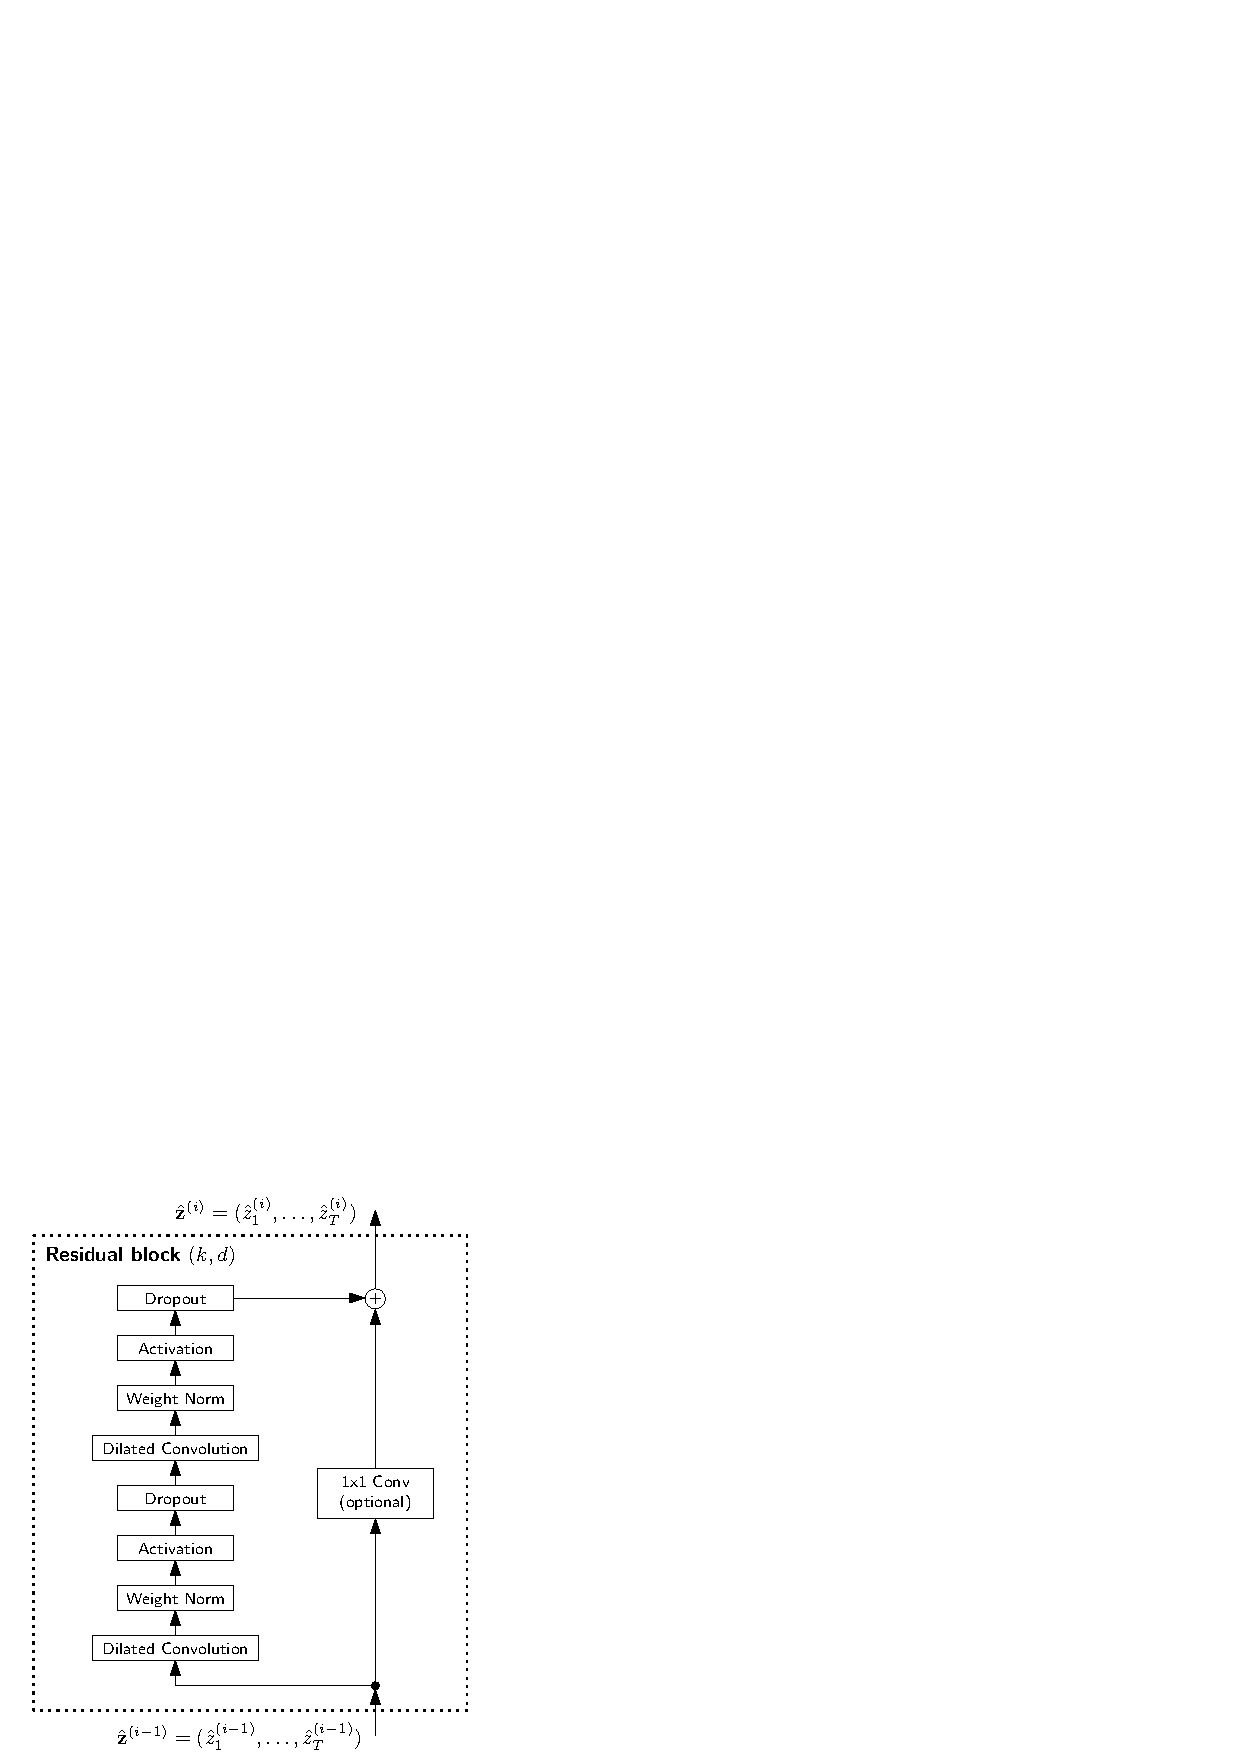
\includegraphics[]{figures/residual_block.pdf}
    \caption{TCN residual block \cite{Bai2018}.}
    \label{fig:residual_block} 
\end{figure}


\begin{itemize}
\item the convolutions are casual, that means no information leakage from future to past (compare to bidirectional RNN).
\item long effective history sizes, i.e., the ability for networks to look very far into the past to make a prediction (receptive field?), by using a combination of very deep networks (augmented with residual layers) and dilated convolutions 
\item this allows layers to learn modifications to the identity mapping rather than the entire transformation, which has been shown to benefit deep neural networks (where?)
\item within a residual block there exist two layers of dilated causal convolution and a rectified linear unit (ReLU) \cite[Nair2010]{Nair2010} as a non-linearity
\item for normalization a weight normalization \cite[Salimans2016]{Salimans2016} is applied to the convolutional filters 
\item additionaly spatioal dropout \cite[Srivastava2014]{Srivastava2014} is added after each dilated convolution for regularization (at each training step, a whole channel is zeroed out)
\item The TCN architecture appers not inly more accurate than canonical recurrent networks such as LSTMs and GRUs, but also simpler and clearer.
\end{itemize}


\subsubsection{Trellis Networks}
\begin{figure}[htbp]
\centering
\includegraphics[scale=1.0]{figures/trellis_net_atomic_level.pdf}
\caption{TrellisNet at an atomic level.}
\label{fig:TrellisNetAtomic}
\end{figure}    

\begin{itemize}
\item[\textbf{Input:}] $x_{1:T} = x_1, \dots, x_T, \quad x_t \in \mathbb R^p, \quad x_{1:T} \in \mathbb R^{T \times p}$ \vspace{0.5em}\\ 
with sequence length  $T$  input dimensionality  $p$
\item[\textbf{Output:}] $y_{1:T} = y_1, \dots, y_T = G(x_1, \dots, x_T)$ \vspace{0.5em} \\
with function $G: \mathcal X^T \rightarrow \mathcal Y^T$ 
\item[\textbf{Hidden:}] $z_t^{(i)} \in \mathbb R^q$
\end{itemize}




\paragraph{LogSoftmax:}

A LogSoftmax normalization is added the last layer of the neural network to obtain the log-probabilities for the differnent classes.
\begin{align}
\text{LogSoftmax}(x_i) = \log\left(\frac{\exp{(x_i)}}{\sum_j \exp(x_j)}\right)
\end{align} 



\subsection{Performance Measure}

\paragraph{Loss Function}
Cross entropy is defined for two probability distributions $p$ and $q$ as
\begin{align}
H(p,q) = - \sum_{x \in \mathcal X} p(x) \log q(x).
\end{align} 
In machine learning cross entropy can be used as a loss funciton to measures the performance of a classification model. The probability $p_{i}$ is the true label (binary indicator 0 or 1), where as the distribution $q_{i}$ is the predicted value of the current model. 


\subsection{Regularization Techniques}


\subsection{Optimization}

\begin{itemize}
\item Regularization with Dropout or Weight Decay
\item check out cyclical learning rates \cite{Smith2017}[Smith2017]
\end{itemize}


Estimate generalization error with a validation set during training. Stop training when the error on the validation set rises (early stopping).


\subsection{Hyperparameter Optimization}

\begin{itemize}
\item optimzie hyperparameters with nevergrad
\item instrumentation: turn a piece of code with parameters into a function defined on an n-dimensional continous data space
\end{itemize}


\subsection{Multi Task Learning}

\begin{itemize}
\item It is the information in these extra training signals that helps the hidden layer learn a better internal representation for the door recognition domain, and this better representation in turn helps the net better learn to recognize [Caruana1997]
\item Information in the extra tasks is helping the hidden layer learn a better internal representation
\item 
\end{itemize}



\subsection{Valididation}

\paragraph{Test set method} Split the observarions into to disjunct subsets 
\begin{align*}
\text{observations}
\begin{cases}
    \text{ training data } \left\{ \left(\mathbf x^{(\alpha)}, \,\mathbf y_T^{(\alpha)}\right) \right \}, \, \alpha \in \{1,\dots, p\} & \\ 
    \;\rightarrow E^T \text{ selects model parameters} & \\  \\
    \text{ test data } \left\{ \left(\mathbf x^{(\beta)}, \,\mathbf y_T^{(\beta)}\right) \right \}, \, \beta \in \{1,\dots, q\} & \\    
    \;\rightarrow \widehat{E}^G \text{ estimates generalization error} & \\ 
\end{cases}
\end{align*} 

\paragraph{n-fold cross-validation} 




\newpage
\section{Beat Tracking System}

From an overall perspective, the proposed automatic beat tracking system comprises three major phrases: data preprocessing, feature learning and temporal decoding. 

\begin{figure}[htbp]
\centering
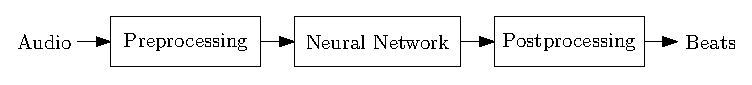
\includegraphics[scale=1.0]{figures/beat_tracking_system.eps}
\caption{Beat tracking system signal flow}
\label{fig:}
\end{figure}  


Seuqence-to-sequence prediction:
\begin{itemize}
\item the entire input sequence can be used to predict each output (not feasible in real time processing)
\end{itemize}

Binary classification problem:
\begin{itemize}
\item beat (class 1)
\item no beat (class 0)
\end{itemize}



\subsection{Dataset}
For training and evaluation we use the datasets listed in Table \ref{tab:datasets}.

The Hainsworth dataset \cite{Hainsworth2004} contains 222 musical audio files, with the following genre breakdown: Rock/Pop (68), Dance (40), Jazz (40); Classical (30), Folk (22), and Choral (22). Each file is between $30$ and $60\,\text{s}$ in length, mono and sampled at $44.1\,\text{kHz}$ with $16\text{-bit}$ resolution.
\begin{table}[htbp]
\caption{Datasets used for training.}
\label{tab:datasets}
\centering

\begin{tabular}{lrr}
\hline

\hline
\textbf{Dataset} & \textbf{files} & \textbf{length} \\
\hline
    Ballroom \cite{Gouyon2006b, Krebs2013} & $685$ & $5\,\text{h} \;57\,\text{m}$\\
    GTZAN \cite{Tzanetakis2002b, marchand2015swing} & $1000$ & $8\,\text{h}\;20\,\text{m}$\\
    Hainsworth \cite{Hainsworth2004} & $222$ & $3\,\text{h}\;19\,\text{m}$\\
    SMC \cite{Holzapfel2012} & $217$ & $2\,\text{h}\;25\,\text{m}$\\    
\hline
    Total & $ $ & $ \,\text{h}\; \,\text{m}$\\  
\hline

\hline
\end{tabular}
\end{table}  


\begin{itemize}
\item The ideal outcome of the annotation is an unambigous representation of the start points of musical events
\item Due to uncertainties in the annotation process, for many types of inpit signals (especially multi-instriment exerpts) it may not possible to determine onset locations with greater precision than $50\,\text{ms}$. \cite{Leveau2004}
\item The input data format is uncompressed linear pulse code modulated (PCM) signals. Single channel $16\,\text{bit}$ linear PCM with a sampling rate of $44100\,\text{Hz}$. The data is created by averaging the two channels of the original stereo recordings.
\end{itemize}


\subsection{Data Preprocessing}

\begin{itemize}
\item ``Is it important to use several features?'' [Durand2015]
\item Two different types of input features: Onset events and harmonic changes
\item Assumtion: Most harmonic changes occur inside a piece of music are located at metric bars \cite[Khadkevich2012]{Khadkevich2012}
\item in complex polyphonic mixtures of music, simultaneously occurring events of high intensities lead to masking effects that prevent any observation of an energy increase of a low intensity onset. To circumbent thesse masking effects, detection functions were proposed that analyze the signal in a bandwise fashion to extract transients occurring in certain frequency regions of the signal [Grosche2011]
\end{itemize}


% https://musicinformationretrieval.wordpress.com/2017/04/25/audio-beat-tracking-human-annotation-strategies/

The Beat Tracking task requires annotations in the form of time instants of beats from a musical excerpt. Additionally, the tempo, metrical level of the beat and downbeat positions can also be annotated for related tasks like downbeat tracking/ meter tracking/ tempo tracking etc.

The method for obtaining ground truth annotations depends on whether the aim is to identify descriptive beat locations or to replicate a human tapping response. In the former case, an initial estimate of the beat locations can be obtained by recording tap times for a given musical excerpt and iteratively modifying and auditing the obtained beat positions while in the latter case, the ground truth can be completely defined by the tapping response \cite{Davies2009b}.

The audio excerpt in time domain and its spectrogram can be visualised using tools like Sonic Visualizer. Beat locations can first be obtained by recording the tap locations the musical excerpt and then manually correcting these locations for exact onsets.  Annotators can also follow a semi-automatic process, for example in [2], where beats and downbeats were first obtained through the ircambeat software and then errors were manually corrected by human annotators.

After preprocessing the audio we obtain the observation set $ O = \left\{ \mathbf x^{(\alpha)}, \,\mathbf y_T^{(\alpha)} \right \}_{\alpha = 1}^p$, with $p$ samples in total. 

\begin{itemize}
\item Data augmentation (transformation or adding noise) $\Rightarrow$ prediction gets robust against transformation and noisy signals
\item output: $y$ probability of beat instant per time frame 
\end{itemize}



The first step in the approach consists of preprocessing the original data. Data preprocessing refers to all transformations on the raw data before the resulting training set is fed to the machine learning algorithm. It includes different methods such as normalization, transformation and feature extraction. 

The data set contains raw pulse code modulated (PCM) audio signals stored as WAV files. For the sake of consistency and also to reduce computational complexity the audio signal is resampled at a sampling rate $f_s = 44.1 \,\text{kHz}$ and converted to a monaural signal by averaging both stereo channels. 


\begin{itemize}
\item Slice audio $x(t)$ into frames $x_n(t)$, $n = 1, 2,\dots, N$, where $N$ is the number of frames
\item Compute complex spectrogram $X(n,k)$ with FFT 
\item Complex spectrogram is converted to the power spectrogram $S(n, k) = |X(n, k)|^2$
\item Mel-spectrogram $M(n,m) = \log \left( S(n,k) \cdot F(m,k)^T + 1.0 \right)$
\end{itemize}
\vspace{1em}

Short-time Fourier transform:
\begin{align}
X(n,k) = \sum_{m = 0}^{N-1} w(m) \, x(m + n  h) \, e^{-2 \pi j  k /N}
\end{align} 

Spectrogram: 
\begin{align}
S(n,k) = |X(n,k)|^2
\end{align} 

Separation of magnitude and phase:
\begin{align} 
X(n,k) = |X(n,k)| \, e^{\, j \phi(n,k)}
\end{align} 


\subsubsection{Chroma Representation}

\begin{itemize}
\item Chords are more likely to change in beat times than on other positions. Chords are more likely to change at the beginnings of measures than at other positions of the beat.
\item A chromagram comprises a time-series of chroma vectors. which represent harmonic content at a specific time in the audio.
\item Chromagrams are concise descriptors of harmony because they encode tone quality and neglect tone height.
\item CRP (chroma DCT-reduced log-pitch) features have significant amount of robustness to changes in timbre an instrumentation \cite[Mueller2010]{Mueller2010}
\item Employ data-driven approach to extract chromagrams that specifically encode content relevant to harmony 
\item Chroma features are noisy in their basic formulation be- cause they are affected by various interferences: musical instruments produce overtones in addition to the funda- mental frequency; percussive instruments pollute the spec- trogram with broadband frequency activations (e.g. snare drums) and/or pitch-like sounds (tom-toms, bass drums); different combinations of instruments (and different, pos- sibly genre-dependent mixing techniques) create different timbres and thus increase variance [7,20] \cite{Korzeniowski2016}
\end{itemize}


\subsection{Feature Learning}



\subsection{Temporal Decoding}

We use a probabilistic dynamic model to exploit the seqential structure of music, generally resulting in a more robust estimation.

As a postprocessing step we make use of a dynamic Bayesian network (DBN) which jointly infers tempo an phase of the beat.

\vspace{1em}
Hidden variables: 
\begin{itemize}
\item $\omega$ - the tempo
\item $\phi$ - the position inside the beat period
\end{itemize}

\vspace{1em}
In order to infer the hidden variables from an audio signal, we specify three entities:

\begin{itemize}
\item \textbf{transition model}: describes the transitions between the hidden variables 
\item \textbf{observation model}: takes the beat activations from the neural network
\item \textbf{initial distribution}: encodes prior knowledge about the hidden variables
\begin{itemize}
\item test probability model for given tempo estimation 
\end{itemize}
\end{itemize}

\subsubsection{Transition Model}
\begin{itemize}
\item The number of observations $M$ per beat at tempo $T$ in BPM is defined as 
\begin{align}
M(T) = \dfrac{60}{T} \,f_r \quad \left[ \dfrac{\text{frames}}{\text{beat}}\right]
\end{align} 
\item The beat position state is dependent on the tempo by using exactly one  state per audio frame.


% \item The beat period is discretized into $\Phi = 640$ equidistant cells
\item $\Phi \in \{1,2,\dots, M(T)\}$ denotes the position inside the beat period (pib)
\item The tempo space corresponds to integer valued beat positions in the interval $[M(T_{\text{max}}), M(T_{\text{min}})]$, with 
\begin{align}
N_{\text{max}} = M(T_{\text{min}}) - M(T_{\text{max}}) + 1
\end{align} 
different tempo states.

% \item For the position inside the beat period we have the following recurrence relation
% \begin{align}
% \phi_k = (\phi_{k-1} + \omega_{k-1} -1) \mod \Phi + 1
% \end{align}  
% \item The tempo space is also discretized tempos between 56 and 216 BPM 
% \begin{align}
% \text{BPM} = \omega \times 60 \times f_r \,/ \, \Phi
% \end{align} 
\item The tempo in beat positions per time frame $\dot \Phi \in \{M(T_{\text{max}}), M(T_{\text{max}}) + 1,  \dots, M(T_{\text{min}})\}$ 
\item For example: 
\begin{align*}
T_{\text{min}} = 56 \,\text{BPM} & \;\rightarrow \; M(T_{\text{min}}) = 107 \\
T_{\text{max}} = 215 \,\text{BPM} &\;\rightarrow \; M(T_{\text{max}}) = 28 
\end{align*} 
\vspace{-1.5em}
\begin{align*}
&\Phi \in \{1, 2, \dots ,107\} \\
&\dot \Phi \in \{28, 29, \dots ,107\}
\end{align*} 


\item Transitions to each tempo is allowed but only at beat times
\begin{align}
\omega_k = 
\begin{cases}
\omega_{k-1}, & P(\omega_k|\omega_{k-1}) = 1 - p_\omega \\
\omega_{k-1}+1, & P(\omega_k|\omega_{k-1}) = \frac{p_\omega}{2} \\
\omega_{k-1}-1, & P(\omega_k|\omega_{k-1}) = \frac{p_\omega}{2} \\
\end{cases}
\end{align} 
\item The probability of tempo change is heuristically set to $p_\omega = 0.002$
\item Higher-level or domain specific knowledge could be used to set this parameter. For example in rock or pop music, the beat is usually quite steady, so a samll value for $p_\omega$ would be quite appropriatre, while for classical music, particularly styles including many tempo changes, a higher value would be more optimal.
\end{itemize}




\subsubsection{Observation model}




% \subsection{Time-Frequency Reassignment}
% \begin{itemize}
% \item audio signals have a distribution of energy that varies in time and frequency
% \item a spectrogram is constrained by an unfortunate tradeoff between resolution in time and frequency
% \item time-frequency reassignment: mapping the data to time-frequency coordinates that are nearer to the true region of support of the analyzed signal
% \item time-frequency reassignment has been used in a variety of applications for obtaining improved time and frequency estimates for time-varying spectral data [cite... 16-18]
% \end{itemize}

% \paragraph{Potential features:} Zero Crossing Rate, Energy, Danceability, Entropy of Energy, Spectral Centroid, Spectral Spread, Spectral Entropy, Spectral Flux, Spectral Roll off, MFCC, Chroma Vector, Chroma Deviation


% \section{Clustering}
% The whole training data gets separated in different clusters. Each cluster represents a homogenous subset of the whole data set, i.e., the multiple models are trained for specific aspects (e.g. genre, timbre, rhythmical patterns, instrumentation, etc.). 

% basic principles of how humans understand rhythms









\newpage
\section{Evaluation}

% Discontinuity in the pulse see Gouyon2005 page 3

\begin{itemize}
\item annotations tapped at different metrical levels in beat tracking
\item a evaluation method should adequately contend with the inherent uncertainty and/or ambiguity while providing a measurement of performance which is both meaningful and easy to interpret. \cite{Davies2009b}
\item objective methods for beat tracking evaluation compare the output beat times from a beat tracking algorithm against one or more sequences of ground truth annotated beat times. \cite{Davies2009b}
\item We must question the imprtance of strict continuity when evaluating a beat tracking system. A single misplaced beat, in the context of a sequence of otherwise accurate beats, is a far less disturbing error than the accuracy calculated with the ontinuity requiremet would suggest. 
\end{itemize}


\subsection{Performance measures}

Set of annotated beat times $\mathcal A = \{a_1, \dots, a_A\}$ \\
Set of predicted beat times $\mathcal B = \{b_1, \dots, b_B\}$ \\

True positive if beat is in $\pm 70\,\text{ms}$ rage of annotated beat

$tp =$ number of true positives \\
$fp =$ number of false positives (extra detections) \\
$fn =$ number of false negatives (missed detections) 

\paragraph{Precision and recall:} $ $

$\text{precision} = \dfrac{tp}{tp + fp}\;, \qquad \text{recall} = \dfrac{tp}{tp + fn}$


\paragraph{F-measure:} $ $

$F_1 = 2 \cdot \dfrac{\text{precision} \cdot \text{recall}}{\text{precision} + \text{recall}} = \dfrac{2\, tp}{2\, tp + fp + fn}$

\paragraph{P-score:} Define two sequences $T_a$ and $T_b$ as 

$T_a(n) = \begin{cases}
	1, &\text{ if } n \in \mathcal A \\
	0 , & \text{ otherwise }
\end{cases}, \qquad T_b(n) = \begin{cases}
	1, &\text{ if } n \in \mathcal B \\
	0 , & \text{ otherwise }
\end{cases}$

$\text{P-score} = \dfrac{\displaystyle \sum_{m=-w}^w  \sum_{n}\,  T_a(n)\,  T_b(n+m)}{\max(A,B)} \;, \qquad \text{where } w = 0.2 \, \text{median}(\Delta_a)$ 



\subsection{Saliency maps}

\begin{itemize}
\item Artificial neural networks often give good results, but it is difficult to understand what they learned, or on which basis they generate their output.
\item compute saliency maps using guided back-propagation [25]
\end{itemize}



\subsection{Network training}

\begin{itemize}
\item To achieve better results, we could use DNN ensembles instead of a single DNN. We could ensure that the network sees data for which its pre- dictions are wrong more often during training, or similarly, we could simulate a more balanced dataset by showing the net super-frames of rare chords more often \cite{Korzeniowski2016}
\end{itemize}



\subsection{Labeling}

\begin{itemize}
\item In an editor (Sonic Visualizer) that enables a user to mark beat positions in a digitalized audio signal while listening to the audio and watching its waveform.
\item The positions can be finely adjusted by playing back the audio with click tones at beat times.
\end{itemize}


\section{Conclusion}

\begin{itemize}
\item We have presented an efficient audio based beat tracking algorithm able to produce equivalante results to the current state-of-the-art. 
\item Limitations in both the amount of training data and the variable quality of the annotations. Perform data augmentation. 
\item Dataset size: ``\emph{[...] a rough rule of thumb is that a supervised deep learning algorithm will gernerally achieve acceptable performance with around 5000 labeled examples per category and will match or exceed human performance when trained with a dataset containing at least 10 million labeled examples.}'' \cite[Goodfellow2016]{Goodfellow2016}
\end{itemize}

\newpage

\section{Appendix}

\subsection{Hyperparameter} 
\begin{itemize}
\item window function (e.g. Hamming window)
\end{itemize}

\newpage 
\bibliographystyle{unsrt}
\bibliography{references}

\end{document}